As implemented for ProtoDUNE-SP, a fully loaded WIB (one WIB plus four FEMBs) requires
12~V and draws up to approximately 4~A. The full electronics for one APA (one PTC, five WIBs, and 20 FEMBs) 
requires 12~V and draws approximately 20~A, for a total power of approximately 240~W, as 
described in Section~\ref{sec:fdsp-tpc-elec-design-warm}. The DUNE implementation should require much 
less power as the FPGA will be replaced by the COLDATA chips.

As the LV power is delivered at 48~V to the PTC, each LV power mainframe is chosen to have 
roughly 30-60~V, 13.5~A, 650~W maximum capacity per APA. Using 10AWG cable, a 0.8~V drop is 
expected along the cable with a required power of 306~W out of 650~W available.  
This leaves a significant margin that allows for larger distances between the power supplies and 
the warm interface crates than the $\sim$20~meters in ProtoDUNE-SP.

Four wires are used for each module; two 10AWG, shielded, twisted-pair cables for the power and return; and two 20AWG, shielded, twisted-pair cables for the sense.
The primary protection is the over-current protection circuit in the low voltage supply modules, 
which is set above the $\sim$20~A current draw of the WEIC.  Secondary sense line fusing is 
provided on the PTC.  The LV power cable uses FCi micro TCA connectors, shown in
Figure~\ref{fig:tpcelec-power_conn}.

\begin{dunefigure}
[FCi micro TCA power connector at the PTC end of the cable.]
{fig:tpcelec-power_conn}
{FCi micro TCA power connector at the PTC end of the cable.}
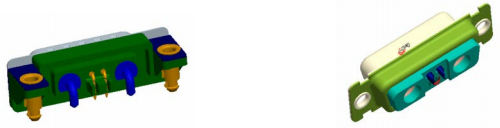
\includegraphics[width=0.9\linewidth]{tpcelec-power_connector.png}
\end{dunefigure}

Bias voltages for the APA wire planes, the electron diverters, and the last field cage electrodes are generated by supplies which are the responsibility of the TPC Electronics consortium.  The current from each of these supplies is expected to be very close to zero in normal operation.  However, the ripple voltage must be carefully controlled to avoid injecting noise into the front-end electronics.  RG-58 coaxial cables connect the wire bias voltages from the mini-crate to the standard SHV
connectors machined directly into the CE feedthrough, so there is no electrical connection between 
the LV power and data connectors and wire bias voltages.

Optical fibers are used for all connections between the WIECs, which act as
Faraday-shielded boxes, and the DAQ and slow control systems.  Duplex LC optical fibers
transmit the one GIG-E connection from each WIB to the slow control system.  The WIB reports
its onboard temperature and the current draw from each FEMB to the slow control system, while the
current draw for each APA is monitored at the mainframe itself.
